\section{Initial conditions}

We need to determine the initial shape of a bubble floating at a gas-liquid interface before it's film ruptures. This derivation is based on the work done in \cite{toba1959drop}.
We are considering the case where the fluid is stationary, i.e. $\bf{u} = \bf{0}$, meaning on the boundaries we only need to consider the Young-Laplace equation:
\begin{align}
    \Delta p=-\gamma \nabla \cdot \hat n
\end{align}

\begin{figure}[hb]
    \centering
    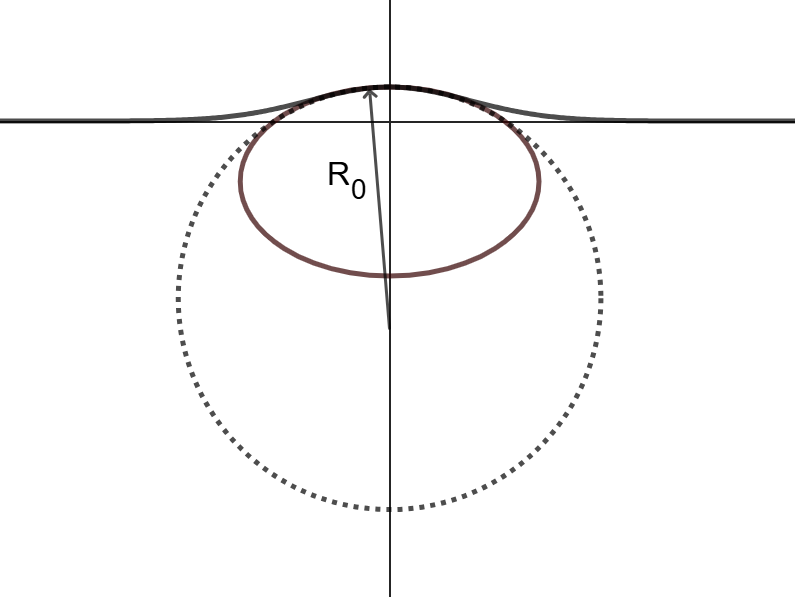
\includegraphics[width=0.55\linewidth]{WriteUp/images/bubble at surface.png}
    \caption{A bubble floating at a surface}
    \label{fig:1}
\end{figure}

We can divide the surface of a bubble into three regions: (A) the submerged portion of the interface, (B) the thin film over the top of the bubble separating the two gas regions, (C) the regions of the interface trailing away from the border of the thin film. We neglect the thickness of the film means we can ignore the weight of the film. Adding that the difference between the gas pressures inside and out of the bubble is uniform, the thin film can be treated as a spherical surface of radius $R_0$. The force balance equations at any point on these surfaces are,
\begin{align}
    (\rho-\rho')gz = \gamma(\frac{1}{R_1}+\frac{1}{R_2}-\frac{4}{R_0})
\end{align}
for region (A),
\begin{align}
    p=p_0 + \frac{4\gamma}{R_0}
\end{align}
for region (B),
\begin{align}
    (\rho-\rho')gz = \gamma(\frac{1}{R_1}+\frac{1}{R_2})
\end{align}
for region (C) where $\gamma$ represents surface tension of the liquid, $g$ is acceleration due to gravity, $\rho$ and $\rho'$ are the densities of the liquid and gas respectively, $p$ and $p_0$ are the gas pressure inside and outside the bubble respectively, $g$ is acceleration due to gravity and $z$ is the height above the still gas liquid interface in the far field. $R_1$ and $R_2$ are the princple radii of curvature of the surface at a point